\documentclass[times, utf8, seminar, numeric]{fer}
\usepackage{ booktabs, tabularx, float, mdframed, graphicx, subcaption, url, listings, caption}
\usepackage{algorithm}
\newenvironment{packed_item}{
	\begin{itemize}
   }{\end{itemize}}
\newenvironment{packed_enum}{
   \begin{enumerate}
   }{\end{enumerate}}

\lstset{ 
  backgroundcolor=\color{white},   % choose the background color; you must add \usepackage{color} or \usepackage{xcolor}; should come as last argument
  basicstyle=\footnotesize,        % the size of the fonts that are used for the code
  breakatwhitespace=false,         % sets if automatic breaks should only happen at whitespace
  breaklines=true,                 % sets automatic line breaking
  captionpos=b,                    % sets the caption-position to bottom
  escapeinside={\%*}{*)},          % if you want to add LaTeX within your code
  extendedchars=true,              % lets you use non-ASCII characters; for 8-bits encodings only, does not work with UTF-8
  frame=single,	                   % adds a frame around the code
  keepspaces=true,                 % keeps spaces in text, useful for keeping indentation of code (possibly needs columns=flexible)
  keywordstyle=\color{blue},       % keyword style
  stepnumber=2,                    % the step between two line-numbers. If it's 1, each line will be numbered
  language=C++,
  basicstyle=\footnotesize,% basic font setting
  }



\begin{document}
% TODO: Navedite naslov rada.
\title{Poravnanje parova sekvenci korištenjem HMM}

% TODO: Navedite vaše ime i prezime.
\author{Petra Dunja Grujić Ostojić , Tea Čutić}

% TODO: Navedite ime i prezime mentora.
\voditelj{izv. prof. dr. sc. Mirjana Domazet-Lošo}

\maketitle

\tableofcontents

\chapter{Uvod}
Jedan od najtežih, a time i najistraživanijih, problema u području bioinformatike je problem poravnanja dviju sekvenci. Poravnanje je ključan korak u uspoređivanju i analizi DNA, RNA i proteinskih sekvenci te omogućuje uvid u zajedničke evolucijske korijene ili indikatore genetskih bolesti.

\bigskip

Ovaj rad bavi se implementacijom algoritma za poravnanje koji koristi skrivene  Markovljeve modele (eng. Hidden Markov Models - HMM). Skriveni Markovljevi modeli su probabilistički modeli korišteni za predstavljanje stohastičkih procesa. Ovaj model sastoji se od više različitih stanja koja, u kontekstu modeliranja odnosa dvaju znakovnih nizova, mogu predstavljati stanja podudaranja, umetanja i brisanja. Vezama između tih stanja označene su vjerojatnosti prelaska iz jednog stanja u drugo ili ostanka u istom stanju. Za dobivanje inicijalne procjene parametara modela HMM korištena je javno dostupna baza poravnanja HIV sekvenci \footnote{https://www.hiv.lanl.gov/content/sequence/NEWALIGN/align.html}. U ovom su radu korištena tri algoritma: Baum-Welch algoritam, Viterbijev algoritam te Needleman-Wunsch algoritam. Od navedenih algoritama, za algoritme Baum-Welch i Viterbi pisana je vlastita implementacija dok je algoritam Needleman-Wunsch preuzet iz javno dostupnog izvora te se koristi za procjenu kvalitete poravnanja kojeg dobijemo u našim rezultatima.

\bigskip

Drugo poglavlje rada bavi se detaljnijim opisom algoritama Baum-Welch i Viterbi. Treće poglavlje bavi se analizom dobivenih rezultata te njihovom usporedbom s rezultatima dobivenima s pomoću algoritma Needleman-Wunsch.







\chapter{Opis algoritama}

\section{Baum-Welch algoritam}
Baum-Welch algoritam, poznat i kao algoritam "forward-backward", je iterativni postupak koji se koristi za treniranje skrivenih Markovljevih modela odnosno za procjenu njegovih parametara pi, A i E. A je matrica vjerojatnosti prijelaza između stanja modela, E je matrica vjerojatnosti emisije simbola x u nekom stanju y, a pi je vektor početnih vjerojatnosti stanja. Algoritam se sastoji od tri koraka, inicijalizacije parametara HMM, računanje očekivanja te maksimizacije očekivanja. Implementacija algoritma rađena je po uzoru na paket HMM iz R-a \footnote{\url{https://rdrr.io/cran/HMM/src/R/HMM.r}}. 

\bigskip
Ulaz u Baum Welch algoritam je HMM s postavljenim inicijalnim vrijednostima navedenih parametara, niz parova simbola, vrijednost delta te zadani broj iteracija. Parametri HMM-a mogu se inicijalizirati nasumično, a u ovom smo ih radu procijenili na uzorku od 500 sekvenci odnosno 249 500 parova sekvenci. Prije inicijalizacije te prije pokretanja algoritma potrebno je obraditi sekvence. Najprije se izbace sve sekvence koje sadrže bilo koje znakove koji nisu znakovi A,C,T,G i -.  Iz parova sekvenci potrebno je izbaciti praznine ako se one nalaze na istom indeksu u svakoj od sekvenci te uzastopne praznine (npr. sekvence -AG i C-T postaju AG i CT). Zatim je potrebno napraviti listu parova simbola od svakog para sekvenci. Neka imamo par sekvenci ACTA i GCAT pripadajuća lista parova simbola bila bi AG, CC, TA, AT.

\bigskip
Nakon inicijalizacije HMM te pripreme sekvenci za obradu, slijedi iterativno računanje očekivanja te 
njegova maksimizacija. Trajanje algoritma određeno je brojem iteracija x te vrijednosti delta d koje se 
postavljaju proizvoljno. Algoritam može prestati s radom nakon nekog određenog broja iteracija ili se 
nakon svake iteracija može računati vrijednost delta $d_i$. Vrijednost $d_i$ definirana je kao zbroj 
kvadratne razlike početne te izračunate matrice A i kvadratne razlike početne i izračunate matrice E. 
Uvjet zaustavljanja na temelju vrijednosti delte glasi $d_i$ < d, a provjerava se na kraju svake iteracije. 

\bigskip
Unutar svake iteracije provodi se jedan forward i jedan backward algoritam. 
Forward algoritam koristi se za izračun vjerojatnosti da je u trenutku \textit{t}   model u stanju \textit{i}, 
koristeći pri tom znanje o prethodno emitiranim simbolima. 
Rezultat forward algoritma je matrica koju označavamo s $\alpha$. 
Backward algoritam koristi se za izračun $\beta$ matrice koja također izračunava vjerojatnost da je u trenutku \textit{t} model u stanju \textit{i} te da je emitirao \textit{T-t} simbola od trenutka \textit{T} do trenutka \textit{t+1}. Na temelju izračunatih matrica $\alpha$ i $\beta$ dalje računamo vjerojatnosti $\gamma$ i $\xi$. $\gamma$ je posteriorna vjerojatnost da se sustav nalazi u stanju Si u trenutku t za promatrani niz i parametre HMM. $\xi$ je vjerojatnost da se model, u trenutcima \textit{t}  i \textit{t+1} nalazi u stanjima \textit{i} i \textit{j} uz promatrani niz i parametre modela. Na kraju iteracije, s dobivenim matricama $\xi$ i $\gamma$ ažuriramo vrijednosti parametra modela.

\bigskip
Budući da računamo s vjerojatnostima koje se kreću u rasponu od 0 do 1, za računanje se koriste logaritmi te pripadne logaritamske implementacije računskih operacija.
Implementacije funkcija za zbroj i umnožak logaritama prikazane su kodom \k1 (napomena: LOGZERO je varijabla postavljena na broj -INFINITY, a predstavlja broj 0).


\begin{lstlisting}[language=C++, caption={Funkcije za računanje s logaritamskih vrijednostima}, captionpos=b, label={k1}]
double log_sum(double x, double y){
	if (x==LOGZERO || y==LOGZERO){
		if (x==LOGZERO){
			return y;
		} 
		return x;
	} else if (x > y){
		return x + compute_log(1 + compute_exp(y-x));
	} else {
		return y + compute_log(1 + compute_exp(x-y));
	}
}

double log_product(double x, double y){
	if (x==LOGZERO || y==LOGZERO){
		return LOGZERO;
	}
	return x + y;
}
\end{lstlisting}



\section{Viterbi algoritam}
Viterbijev algoritam pronalazi najvjerojatniji niz stanja u skrivenom Markovljevom modelu (HMM) na temelju opaženog niza simbola i parametara modela. Implementirale smo inačicu Viterbijeva algoritma koja pronalazi najvjerojatniji slijed skrivenih stanja na temelju opaženih parova simbola. Ta stanja ujedno predstavljaju poravnanje dva slijeda na ulazu algoritma. 

Naš skriveni Markovljev model može se opisati slikom \ref{fig:hmm}. Razlikujemo 3 skrivena stanja: M, X i Y. U dijelu literature stanje X se naziva $I_{x}$, a stanje Y $I_{y}$ upravo jer predstavlja umetanje (engl. insertion) u odgovarajuću sekvencu. Pretpostavlja se da je početno stanje M. Generiranje nizova ovisi o vjerojatnostima prijelaza između stanja i vjerojatnosti emisije parova simbola. Ovako opisani model ima dva stupnja slobode: vjerojatnost prijelaza (delta) iz stanja M  u X ili Y i vjerojatnost ostanka (epsilon) u stanju X, tj. Y. Ostale vjerojatnosti proizlaze iz činjenice da zbroj izlaznih vjerojatnosti iz svih stanja mora biti 1. 
Stanje M odgovara emisiji para simbola $x_{i}$, $y_{j}$, a stanja X i Y predstavljaju emisiju simbola jedne sekvence i praznine u drugom slijedu. Pomoću Baum Welch algoritma i javno dostupne baze poravnanja HIV sekvenci odredile smo parametre modela. Ovisno o kriteriju zaustavljanja BW algoritma dobivena su 2 HMM modela. Kako bi modeli odgovarali modelu sa slike, za vjerojatnosti prijelaza koje bi trebale biti jednake (primjerice, prijelaz iz M u X i iz M u Y) uzeta je srednja vrijednost i osigurano da je zbroj vjerojatnosti u retku matrice prijelaza jednak 1.
\begin{figure}[H]
	\centering
	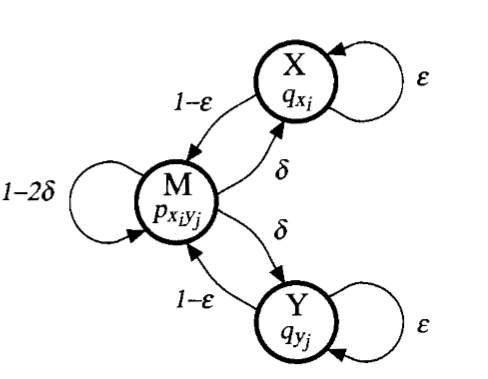
\includegraphics[height=6cm,keepaspectratio]{slike/hmmpair.png} 
	\caption{HMM za poravnanje sljedova, slika preuzeta iz \cite{durbin1998biological}}
	\label{fig:hmm}
\end{figure}

 U nastavku je opisan Viterbijev algoritam. Iterativno se popunjavaju 3 matrice veličine $(n+1) \cdot (m+1)$, pri čemu je $n$ veličina prvog, a $m$ veličina drugog slijeda kojeg želimo poravnati . Inicijalno se postavi: 
 $V^{M}(0, 0) &= 1, V^{I_x}(i, 0) &= 0, V^{I_y}(0, j)} &= 0$.

\begin{algorithm}[H]
		\caption{Viterbijev algoritam}
	\label{alg:viterbi}
	\begin{align*}
		V^{M}(i, j) &= p_{x_{i} y_{j}} \cdot \max \left\{ \begin{aligned}
			&(1 - 2\delta) \cdot V^{M}(i - 1, j - 1) \\
			&(1 - \varepsilon) \cdot V^{I_x}(i - 1, j - 1) \\
			&(1 - \varepsilon) \cdot V^{I_y}(i - 1, j - 1)
		\end{aligned}  \\
		V^{I_x}(i, j) &= q_{x_{i}} \cdot \max \left\{ \begin{aligned}
			&\delta \cdot V^{M}(i - 1, j) \\
			&\varepsilon \cdot V^{I_x}(i - 1, j)
		\end{aligned}  \\
		V^{I_y}(i, j) &= q_{y_{j}} \cdot \max \left\{ \begin{aligned}
			&\delta \cdot V^{M}(i, j - 1) \\
			&\varepsilon \cdot V^{I_y}(i, j - 1)
		\end{aligned} 
	\end{align*}
\end{algorithm}

U praksi su sljedovi koje trebamo poravnati dugački te je navedeni algoritam neupotrebljiv jer je množenje velikog broja vjerojatnosti (brojeva između 0 i 1) numerički nestabilno. Zato smo implementirale logaritamsku inačicu.

\begin{algorithm}
	\caption{Viterbijev algoritam - logaritamska inačica}
	\label{alg:viterbilog}
	\begin{align*}
		\log{V^{M}(i, j)} &= \log{p_{x_{i} y_{j}}} + \max \left\{ \begin{aligned}
			&\log(1 - 2\delta) + \log{V^{M}}(i - 1, j - 1) \\
			&\log(1 - \varepsilon) + \log{V^{I_x}}(i - 1, j - 1) \\
			&\log(1 - \varepsilon) + \log{V^{I_y}}(i - 1, j - 1)
		\end{aligned}  \\
		\log{V^{I_x}(i, j)} &= \log{q_{x_{i}}} + \max \left\{ \begin{aligned}
			&\log{\delta} + \log{V^{M}(i - 1, j)} \\
			&\log{\varepsilon} + \log{V^{I_x}(i - 1, j)}
		\end{aligned}  \\
		\log{V^{I_y}(i, j)} &= \log{q_{y_{j}}} + \max \left\{ \begin{aligned}
			&\log{\delta} + \log{V^{M}}(i, j - 1) \\
			&\log{\varepsilon} + \log{V^{I_y}}(i, j - 1)
		\end{aligned} 
	\end{align*}
	
	
\end{algorithm}
Potrebno je iterativno ažurirati 3 matrice ($V^{M},V^{Ix},V^{Iy}$). Radi se o velikom zauzeću memorije te u slučaju dugačkih sekvenci moguće je da one neće stati u radnu memoriju. Već iz samih jednadžbi može se primijetiti da su nam za izračun vrijednosti u koraku $i,j$ potrebni samo podaci iz prethodnog koraka $i-1, j-1$. Tako da umjesto da pohranjujemo 3 velike matrice možemo iz koraka u korak mijenjati 1 vektor veličine drugog slijeda i pamtiti takav vektor iz prethodnog koraka $i$. U našoj implementaciji element tog vektora je struktura ViterbiInfo koja sadrži 3 broja koja predstavljaju dotadašnju log vjerojatnost za svako skriveno stanje. Zadnji element posljednjeg vektora koji izračunamo predstavlja log vjerojatnost završetka dobivenog poravnanja u stanju M, $I_{x}$ i $I_{y}$. Odredi se najvjerojatnije stanje i rekonstruira se optimalno poravnanje.

Kako bismo rekonstruirali optimalno poravnanje ulaznih nizova $x$ i $y$, potrebno je pamtiti iz kojeg se stanja došlo u najvjerojatnije stanje u svakom koraku. Rekonstrukcija se započinje od kraja. Indeksi $i$ i $j$ se postavljaju na duljinu prvog, odnosno drugog niza. Moguća su 3 slučaja:
\begin{enumerate}
	\item prethodno stanje je M – emitiraj znakove x[i-1],y[i-1] i smanji indekse $i$ i $j$ za jedan
	\item prethodno stanje je $I_{x}$ – emitiraj znak x[i-1] i prazninu u drugu sekvencu, umanji $i$ za jedan
	\item prethodno stanje je $I_{y}$ – emitiraj znak y[j-1] i prazninu u prvu sekvencu, umanji $j$ za jedan
\end{enumerate}
 Postupak se ponavlja dok nisu emitirani svi simboli iz oba ulazna niza.
 
 Viterbijev algoritam primjer je algoritama dinamičkog programiranja jer efikasno rješava problem optimalnog poravnanja sljedova razbijajući ga na manje podprobleme (manje dijelove sljedova) i koristeći njihova optimalna rješenja za konstrukciju globalnog optimalnog poravnanja. Naime, u svakom se koraku računa trenutno najvjerojatnije stanje s obzirom na emitirane simbole i prethodno stanje sustava.


\chapter{Analiza rezultata}
Pomoću algoritma Baum Welch procijenile smo parametre HMM modela koji opisuje poravnanje HIV sljedova. Korištena su 2 kriterija zaustavljanja algoritma: \begin{enumerate}
	\item delta = 0.001, broj iteracija = 100
	\item delta = 0.01, broj iteracija = 100
\end{enumerate}
Pomoću dobivenih modela generirale smo poravnanje nasumično odabranih 50 sljedova. U \cite{durbin1998biological} navode da je primjena Viterbijeva algoritma na HMM modelu ekivalentna algoritmu dinamičkog programiranja za optimalno poravnanje sekvenci kao što je Needleman Wunsch. 

Na odabranim sekvencama provele smo poravnanje pomoću NW algoritma uz 2 kriterija bodovanja poravnanja sljedova:
\begin{itemize}
	\item +2 za podudaranje, -1 za nepodudaranje, -2 za prazninu
	\item +2 za podudaranje, -1 za nepodudaranje, -4 za prazninu
\end{itemize} 

Dobiveni rezultati su prikazani u tablici \ref{tab:rezultati}.

\begin{table}[ht]
	\centering
	\small % Podesite veličinu fonta
	\begin{tabular}{lccc}
		  \toprule
		\textbf{MODEL} & \textbf{BODOVANJE} & \textbf{SREDNJA VRIJEDNOST} & \textbf{STANDARDNA}} \\
		& & \textbf{BODOVANJA} & \textbf{DEVIJACIJA} \\
		\midrule
	
		\midrule
		
		NW & +2, -1, -2 & 15080.90 & 689.12\\
		Viterbi ($\delta$ = 0.01) & +2, -1, -2 & 14487.92 & 737.18 \\
		Viterbi ($\delta$ = 0.001) & +2, -1, -2 & 14555.24 & 722.95 \\
		NW & +2, -1, -4 & 14473.60 & 1179.47 \\
		Viterbi ($\delta$ = 0.01)  & +2, -1, -4 & 13577.40 & 1238.99 \\
		Viterbi ($\delta$ = 0.001) & +2, -1, -4 & 13676.96 & 1211.97 \\
		\bottomrule
	\end{tabular}
	\caption{Srednje vrijednosti bodovanja i standardne devijacije poravnanja modela}
	\label{tab:rezultati}
\end{table}

Može se reći da je model s manjom deltom dao bolja poravnanja: bliži je prosječnom poravnanju Needleman Wunsch algoritma i ima manju standardnu devijaciju. Needleman Wunsch algoritam prosječno je dao bolja poravnanja po obje bodovne sheme. Na slikama 3.1 i 3.2 se može vidjeti odstupanje naših modela od NW algoritma za svaku sekvencu. Za oba modela je to odstupanje od oko 10\% od Needleman Wunsch poravnanja. U slučaju sheme koja manje kažnjava praznine (-2, umjesto -4) odstupanje je malo (razlika oko 2 \%) manje.


\begin{figure}[H]
	\centering
	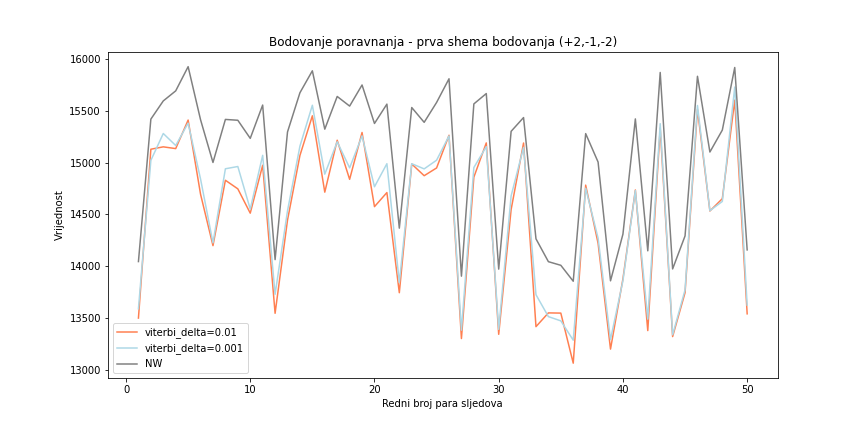
\includegraphics[height = 8 cm, width=0.9\textwidth]{slike/bodovanje_graf1.png} 
	\caption{Usporedba rezultata naših modela i Needleman Wunsch algoritma}}
	\label{fig:bodovanje1}
\end{figure}

\begin{figure}[H]
	\centering
	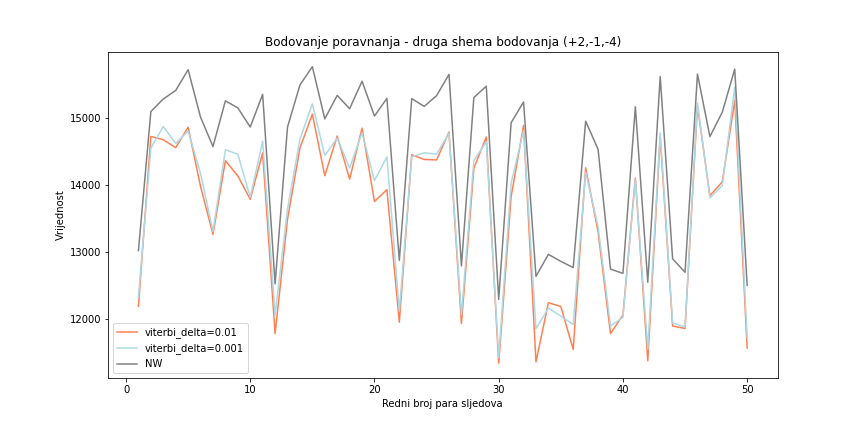
\includegraphics[height = 8 cm, width=0.9\textwidth]{slike/bodovanje_graf2.png} 
	\caption{Usporedba rezultata naših modela i Needleman Wunsch algoritma}}
	\label{fig:bodovanje2}
\end{figure}

Rezultati bi bili bolji da se koristilo više sekvenci za inicijalnu procjenu modela pomoću Baum Welch algoritma. Bilo bi poželjno iskoristiti i sekvence različite od HIVa kako bi model bolje generalizirao. Zbog ograničenih resursa, korišten je manji broj sekvenci za učenje parametara modela i za testiranje Viterbijeva algoritma. Ipak, rezultati su pokazali da je ovaj pristup poravananja blizak rezultatima NW algoritma ukoliko su sekvence koje treba poravnati slične onima koje su korištene za određivanje parametara HMM.

\chapter{Zaključak}
U ovom je radu isprobano poravnanje sljedova HIVa pomoću skrivenog Markovljeva modela. Za određivanje parametara modela korišten je algoritam Baum Welch, a za generiranje poravnanja sljedova Viterbijev algoritam. Dobiveni rezulati su uspoređeni s rezultatima dobivenim algoritmom Needleman Wunsch koji generira globalno optimalno poravnanje sljedova. Ključno poboljšanje dosadašnjeg rada bi bilo korištenje većeg broja sekvenci za procjenu parametara modela te optimizacija vremenske i memorijske složenosti implementacije algoritama.
 
\nocite{*}
\bibliography{literatura}
\bibliographystyle{fer}


\end{document}
